%%%%%%%%%%%%%%%%%%%%%%%%%%%%%%%%%%%%%%%%%%%%%%%%%%%%%%%%%%%%%%%%%%%%%%
% LaTeX Template: Two Column Colour Article
%
% Source: http://www.howtotex.com/
% Feel free to distribute this template, but please keep the
% referal to howtotex.com.
% Date: Feb 2011
% 
%%%%%%%%%%%%%%%%%%%%%%%%%%%%%%%%%%%%%%%%%%%%%%%%%%%%%%%%%%%%%%%%%%%%%%
% How to use overleaf.com: 
%
% You edit the source code here on the left, and the preview on the
% right shows you the result within a few seconds.
%
% You can upload figures, bibliographies, custom classes and
% styles using the files menu.
%
% If you're new to LaTeX, the wikibook is a great place to start:
% http://en.wikibooks.org/wiki/LaTeX
%
%%%%%%%%%%%%%%%%%%%%%%%%%%%%%%%%%%%%%%%%%%%%%%%%%%%%%%%%%%%%%%%%%%%%%%
% adaptions made by wolfgang stoettner mail@stoettner.net
%%%%%%%%%%%%%%%%%%%%%%%%%%%%%%%%%%%%%%%%%%%%%%%%%%%%%%%%%%%%%%%%%%%%%%

%%% Preamble
\documentclass[	DIV=calc,%
							paper=a4,%
							fontsize=11pt,%
							twocolumn]{scrartcl} % KOMA-article class
\usepackage[french]{babel}	% English language/hyphenation
\usepackage[protrusion=true,expansion=true]{microtype}	% Better typography
\usepackage{amsmath,amsfonts,amsthm} % Math packages
\usepackage{pythontex} % Math packages
\usepackage[pdftex]{graphicx} % Enable pdflatex
\usepackage{wrapfig} % enable figure wrapping
\usepackage[svgnames]{xcolor} % Enabling colors by their 'svgnames'
\usepackage[hang, small,labelfont=bf,up,textfont=it,up]{caption} % Custom captions under/above floats
\usepackage{epstopdf} % Converts .eps to .pdf
\usepackage{subfig}	% Subfigures
\usepackage{booktabs} % Nicer tables
\usepackage{fix-cm}	% Custom fontsizes
\usepackage{booktabs} % prof. looking tables (www.en.wikibooks.org/wiki/LaTeX/Tables#Professional_tables)
\usepackage{float}
\usepackage{tgtermes}
\usepackage[export]{adjustbox}
\usepackage[default]{lato}
\usepackage{newtxmath}
\usepackage[T1]{fontenc}
\usepackage[utf8]{inputenc}
\usepackage{stackengine}
\usepackage{tikz,pgfplots}


%%% Custom sectioning (sectsty package)
\usepackage{sectsty} % Custom sectioning (see below)
\allsectionsfont{%		% Change font of al section commands
	\usefont{OT1}{phv}{b}{n}%	% bch-b-n: CharterBT-Bold font
	}

\sectionfont{%		% Change font of \section command
	\usefont{OT1}{phv}{b}{n}%	% bch-b-n: CharterBT-Bold font
	}
%%% Headers and footers
\usepackage{fancyhdr} % Needed to define custom headers/footers
	\pagestyle{fancy} % Enabling the custom headers/footers
\usepackage{lastpage}	

% Header (empty)
\lhead{}
\chead{}
\rhead{\today}
% Footer (you may change this to your own needs)
\lfoot{\footnotesize \texttt{formulaire SysElec} \textbullet \vspace{5pt} Antonin Kenzi}
\cfoot{}
\rfoot{\footnotesize page \thepage\ of \pageref{LastPage}}	% "Page 1 of 2"
\renewcommand{\headrulewidth}{0.0pt}
\renewcommand{\footrulewidth}{0.4pt}
\newcommand{\hformbar}[1]{\bigskip\hrule\vspace{5pt}} % creates a horizontal bar to separate formulae better; space adaptions can be made centrally here


%%% Creating an initial of the very first character of the content
\usepackage{lettrine}
\newcommand{\initial}[1]{%
     \lettrine[lines=3,lhang=0.3,nindent=0em]{
     				\color{DarkGoldenrod}
     				{\textsf{#1}}}{}}

%%% Title, author and date metadata
\usepackage{titling} % For custom titles

\newcommand{\HorRule}{\color{DarkGoldenrod}%	% Creating a horizontal rule
									  	\rule{\linewidth}{1pt}%
										}
\pretitle{\vspace{-30pt} \begin{flushleft} \HorRule 
				\fontsize{15}{15} \usefont{OT1}{phv}{b}{n} \color{DarkRed} \selectfont 
				}
\title{Formulaire SysElec} % Title of your article goes here
\posttitle{\par\end{flushleft}}
\preauthor{\vspace{-20pt} \begin{flushleft}\large \usefont{OT1}{phv}{b}{sl} \color{DarkRed}}
\author{Kenzi Antonin}	% Author name goes here
\postauthor{\vspace{-20pt} \footnotesize \usefont{OT1}{phv}{m}{sl} \color{Black}  \par\end{flushleft}\HorRule}
\date{\vspace{-30pt} \today} % No date
\newcounter{mycounter}
%%% wws: create a non-indented formula name
\newcommand{\formdesc}[1]{\noindent\textbf{#1} \addtocounter{mycounter}{1} \hfill \themycounter}
\newcommand{\formtitle}[1]{\noindent\underline{#1}}

%%% Begin document -----------------------------------------------------------------
\begin{document}
\maketitle
\thispagestyle{fancy} 	% Enabling the custom headers/footers for the first page 
% The first character should be within \initial{}

\formdesc{Rappel : }

\formtitle{Schéma bloc}

{\hfill$ \eta  = \cfrac{R_L}{R_L + R_s}$ \hfill}

\vspace{5mm}

\begin{center}
    
\includegraphics[width = 0.15\textwidth]{img/huitre.png}
\end{center}

\hformbar




\formdesc{Formule Importantes pour les exercices :}

\formtitle{Étage d'entrée :}

Faire un tableau,

$V_{RL} = AD \cdot U_{gMc}$

$SNRQ = 6.02N + 10.8 + 20log(\cfrac{V_{rms}}{2U_{ref}}) $

$V_{rms} = \cfrac{\hat{U}_{RL}}{\sqrt{2}} $

$Pente = \cfrac{\Delta dB}{log_{10}(\cfrac{f_e}{2\cdot f_c})}[dB/dec]$

\begin{tabular}{c|c|c|c|c}
    Cas & Vin1 & Vin1 & Vout1 & Vout2 \\\hline
    1 & 0 & 0 & y1.1 & y1.2 \\\hline
    2 & x & 0 & y2.1 & y2.2 \\\hline
    3 & 0 & x & y3.1 & y3.2 \\\hline
    4 & x & x & y4.1 & y4.2 \\
\end{tabular}

$(Vin(+)-Vin(-)) = \cfrac{VCC-Vref}{G}$

$V_{outD} = Vout1 - Vout2 $

\formtitle{Quantification}


\begin{center}
    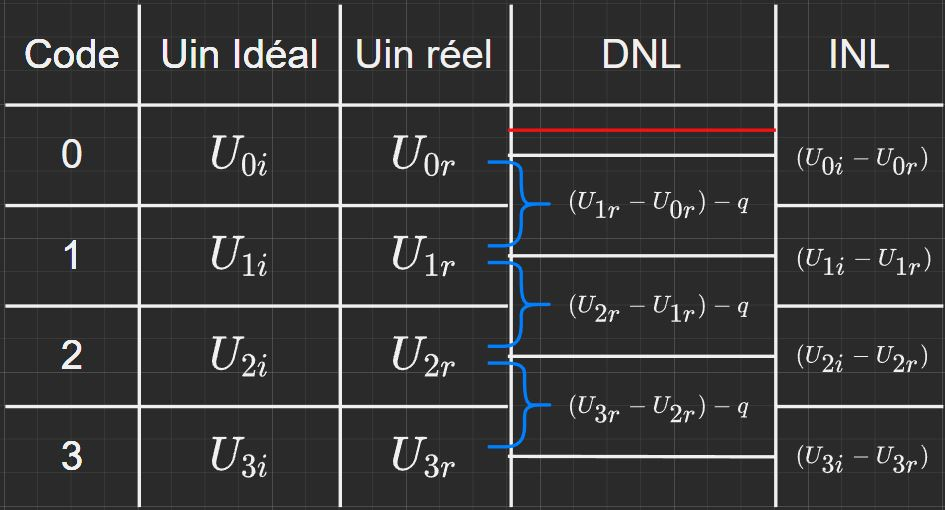
\includegraphics[width = 0.4\textwidth]{img/Table.JPG}
\end{center}



\formdesc{Mode Commun et Différentiel  : }

\begin{enumerate}
    \item Commun : par rapport à la GND
    \item Différentiel : entre deux potentiels 
\end{enumerate}

\formtitle{Schéma bloc}


\vspace{5mm}

\begin{center}
    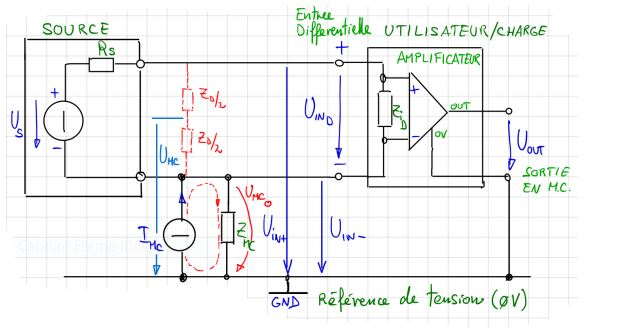
\includegraphics[width = 0.54\textwidth]{img/Schéma.JPG}
\end{center}

Tension mode commun : 
{\hfill$ U_{MC}  = \cfrac{(U_{in+})+(U_{in-})}{2}$ \hfill}

{\hfill$ U_{MC_0}  = I_{MC} \cdot Z_{MC}$ \hfill}

Tension différentielle : 

{\hfill$ U_{D}  = (U_{in+}).(U_{in-})$ \hfill}

\formtitle{Commun Mode Rejection Ratio : CMRR }

Cette grandeur donne l’atténuation d’un signal en entrée en MC sur la sortie :

{\hfill$ CMRR = 20log_{10}\cfrac{U_{in,MC}(f)}{U_{out}(f)}$ \hfill}

\hformbar



\newpage

\hformbar

\formdesc{Méthodologie étage d'entrée}

\hformbar

\formtitle{Superposition : }

Exprimer nœuds par nœuds les potentielles 
Pour définir le gain total et les tensions de référence

\formtitle{Définition de la dynamique :}

La dynamique est la plage de tension sur laquelle il est possible de travailler.

Exemple :

$Av = 5 $

$+vcc = 10 V$

$-vcc = 0 V$

$ Dynamique_{in} = 10/5 = 2 V $ 

\formtitle{Mode Commun :}

$Gain_{reel} = Gain + erreur$

$U_{in\;MC}  = \cfrac{Uin(+) + Uin(-)}{2}$

$Uout_{MC} = \cfrac{Uout(+) + Uout(-)}{2} $  

et garder la composante AC 

\hformbar

\formtitle{Bruit de quantification : }

$SNRQ = 20log(\cfrac{Vrms}{Uref}) + 4.77 + 6.02 * N$\\

$N = \cfrac{SNRQ - 20log(\cfrac{Vrms}{Uref}) - 4.77}{6.02}$

\formtitle{Surechantillionage : }

$\Delta SNRQ = SNRQ1 - SNRQ2$\\

$Nosr = 10^{\cfrac{\Delta SNRQ}{10}}$\\



\formtitle{Filtre d'anti-repliement : }

$Pente = \cfrac{\Delta dB}{20\,log(\cfrac{f_e}{f_c})}$

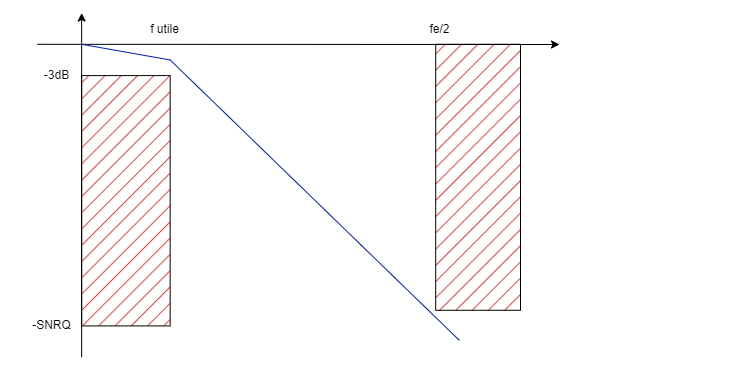
\includegraphics[width = 0.7\textwidth]{Test.drawio.png}


\hformbar


\formtitle{Convertisseur : }

Calcul par étape : 

$Uco_n = Uref \cdot \cfrac{1}{D\#(N-n-1)} - Uin$

Si Uco > 0 alors comparateur à 1 et on ne garde pas le bit $D\#n$

Exemple si $Uco_2$ Et N = 8 et étape 2 mais $D\#5$ :

Si comp = 1 : 

$Uco_3 = Uref \cdot \cfrac{1}{D\#4} - Uin$

Si comp = 0 : 

$Uco_3 = Uref \cdot (\cfrac{1}{D\#5} + \cfrac{1}{D\#4}) - Uin$

\input{chapitre/slide5.tex}

\input{chapitre/slide6.tex}

\input{chapitre/slide7.tex}

\input{chapitre/slide8.tex}

\input{chapitre/slide9.tex}

\input{chapitre/slide10.tex}


\end{document}